\documentclass[12pt]{article}
\usepackage[paper=letterpaper,margin=2cm]{geometry}
\usepackage{amsmath,amssymb,amsfonts}
\usepackage{newtxtext, newtxmath}
\usepackage{enumitem}
\usepackage{titling}
\usepackage{nicematrix}
\usepackage[colorlinks=true]{hyperref}
\usepackage{graphicx}

\setlength{\droptitle}{-6em}

\newcommand{\info}[2]{\frac{#1}{#2}\log\bigl( \frac{#1}{#2} \bigr)}

\begin{document}

\center
Aprendizagem 2023\\
Homework I -- Group 016\\
(ist1100293, ist1102556)\vskip 1cm

\large{\textbf{Part I}: Pen and paper}\normalsize

\begin{enumerate}[leftmargin=\labelsep]
\item Complete the given decision tree using Information gain with Shannon entropy ($\log_2$).
Consider that: i) a minimum of 4 observations is required to split an internal node, and
ii) decisions by ascending alphabetic order should be placed in case of ties.
 
\begin{center}
    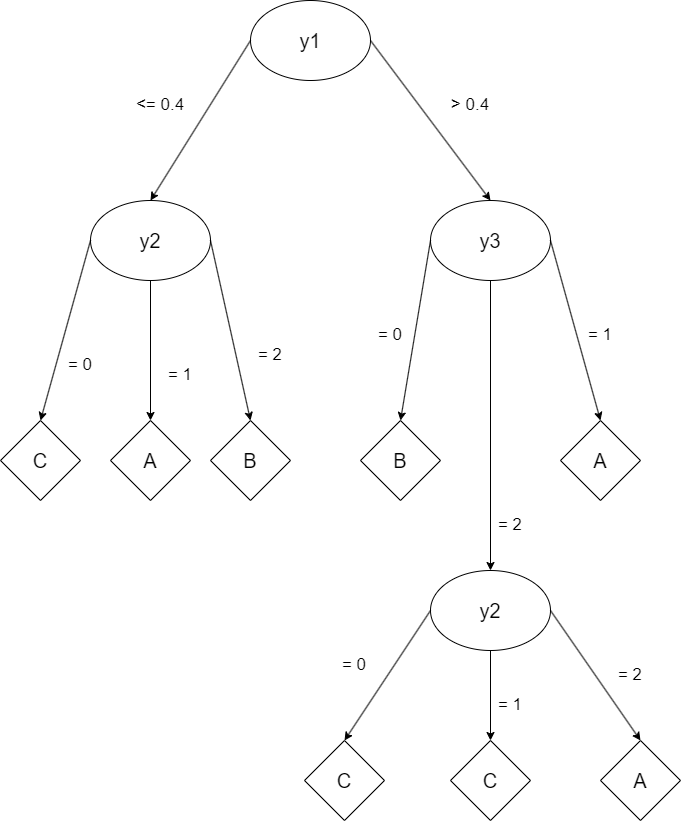
\includegraphics[scale=0.3]{images/decision-tree.png}
\end{center}

\paragraph{For $y_1 > 0.4$}

\begin{equation}
    \begin{split}
        H(y_\textrm{out}) & = -\sum_{v \in y_\textrm{out}}\textrm{p}(v)\log(\textrm{p}(v)) \\
        & = -\info{3}{7} - \info{2}{7} - \info{2}{7} \\
        & \approx 1.5567
    \end{split}
\end{equation}

\begin{equation}
    \begin{split}
        \textrm{IG}(y_\textrm{out}, y_2) &= H(y_\textrm{out}) - H(y_\textrm{out}|y_2) \\
        & = H(y_\textrm{out}) - \sum_{v \in y_2}\textrm{p}(v)H(y_\textrm{out}|y_2=v) \\
        & = H(y_\textrm{out}) - \Biggl( \frac{3}{7}H(y_\textrm{out}|y_2=0) + \frac{2}{7}H(y_\textrm{out}|y_2=1) + \frac{2}{7}H(y_\textrm{out}|y_2=2)\Biggr) \\
        & = H(y_\textrm{out}) - \Biggl( -\frac{3}{7}\biggl( \info{1}{3} + \info{1}{3} + \info{1}{3} \biggr) \\
        & - \frac{2}{7}\biggl( \info{1}{2} + \info{1}{2} \biggr) - \frac{2}{7} \cdot 0 \Biggr) \\
        & \approx 0.5917
    \end{split}
\end{equation}

\begin{equation}
    \begin{split}
        \textrm{IG}(y_\textrm{out}, y_3) &= H(y_\textrm{out}) - H(y_\textrm{out}|y_3) \\
        & = H(y_\textrm{out}) - \sum_{v \in y_3}\textrm{p}(v)H(y_\textrm{out}|y_3=v) \\
        & = H(y_\textrm{out}) - \Biggl( \frac{1}{7}H(y_\textrm{out}|y_3=0) + \frac{2}{7}H(y_\textrm{out}|y_3=1) + \frac{4}{7}H(y_\textrm{out}|y_3=2)\Biggr) \\
        & = H(y_\textrm{out}) - \Biggl( \frac{1}{7} \cdot 0 + \frac{2}{7} \cdot 1 + \frac{4}{7} \cdot 1  \Biggr) \\
        & = H(y_\textrm{out}) - \frac{6}{7} \\
        & \approx 0.6996
    \end{split}
\end{equation}

\begin{equation}
    \begin{split}
        \textrm{IG}(y_\textrm{out}, y_4) &= H(y_\textrm{out}) - H(y_\textrm{out}|y_4) \\
        & = H(y_\textrm{out}) - \sum_{v \in y_4}\textrm{p}(v)H(y_\textrm{out}|y_4=v) \\
        & = H(y_\textrm{out}) - \Biggl( \frac{2}{7}H(y_\textrm{out}|y_4=0) + \frac{3}{7}H(y_\textrm{out}|y_4=1) + \frac{2}{7}H(y_\textrm{out}|y_4=2)\Biggr) \\
        & = H(y_\textrm{out}) - \Biggl( -\frac{2}{7} \cdot 1 - \frac{3}{7}\Bigl( \info{1}{3} + \info{2}{3} \Bigr) - \frac{2}{7} \cdot 1\Biggr)\\
        & \approx 0.5917
    \end{split}
\end{equation}

\paragraph{} For this node $y_3$ has the highest information gain, so we choose it to split the node.

\paragraph{For $y_1 > 0.4 \wedge y_3=2$}

\begin{equation}
    \begin{split}
        H(y_\textrm{out}) & = -\sum_{v \in y_\textrm{out}}\textrm{p}(v)\log(\textrm{p}(v)) \\
        & = -\info{1}{2} - \info{1}{2} \\
        & = 1
    \end{split}
\end{equation}

\begin{equation}
    \begin{split}
        \textrm{IG}(y_\textrm{out}, y_2) &= H(y_\textrm{out}) - H(y_\textrm{out}|y_2) \\
        & = H(y_\textrm{out}) - \sum_{v \in y_2}\textrm{p}(v)H(y_\textrm{out}|y_2=v) \\
        & = H(y_\textrm{out}) - \Biggl( \frac{1}{2}H(y_\textrm{out}|y_2=0) + \frac{1}{4}H(y_\textrm{out}|y_2=1) + \frac{1}{4}H(y_\textrm{out}|y_2=2)\Biggr) \\
        & = H(y_\textrm{out}) - \Biggl( \frac{1}{2} \cdot 0 + \frac{1}{4} \cdot 0 + \frac{1}{4} \cdot 0  \Biggr) \\
        & = H(y_\textrm{out}) - 0 \\
        & = 1
    \end{split}
\end{equation}

\begin{equation}
    \begin{split}
        \textrm{IG}(y_\textrm{out}, y_4) &= H(y_\textrm{out}) - H(y_\textrm{out}|y_4) \\
        & = H(y_\textrm{out}) - \sum_{v \in y_4}\textrm{p}(v)H(y_\textrm{out}|y_4=v) \\
        & = H(y_\textrm{out}) - \Biggl( \frac{1}{2}H(y_\textrm{out}|y_3=0) + \frac{1}{4}H(y_\textrm{out}|y_3=1) + \frac{1}{4}H(y_\textrm{out}|y_3=2)\Biggr) \\
        & = H(y_\textrm{out}) - \Biggl( \frac{1}{2} \Bigl( - \info{1}{2} - \info{1}{2} \Bigr) + \frac{1}{4} \cdot 0 + \frac{1}{4} \cdot 0  \Biggr) \\
        & = H(y_\textrm{out}) - \frac{1}{2} \\
        & = \frac{1}{2}
    \end{split}
\end{equation}

\paragraph{} For this node $y_2$ has the highest information gain, so we choose it to split the node.

\item Draw the training confusion matrix for the learnt decision tree.

\begin{center}

    \begin{table}[htbp]
    \centering
    \begin{NiceTabular}{*{4}{c}*{6}{p{1cm}}}[hvlines]
    \Block{2-2}{} & & \Block{1-3}{Real}\\
    & & A & B & C\\
    \Block{3-1}{Predicted}& A & 4 & 1 & 0\\
    & B & 0 & 2 & 0\\
    & C & 0 & 1 & 4\\
    \end{NiceTabular}
    \end{table}

\end{center}



\item Identify which class has the lowest training F1 score.



\item Considering $y_2$ to be ordinal, assess if $y_1$ and $y_2$ are correlated using the Spearman coefficient.
\begin{center}
    
    \begin{tabular}{|c | c | c | c | c|}
        \hline
        D & $y_1$ & $r_{y_1}$ & $y_2$ & $r_{y_2}$\\
        \hline
        $x_1$    & 0.24 & 3  & 1 & 8 \\
        $x_2$    & 0.06 & 2  & 2 & 11 \\
        $x_3$    & 0.04 & 1  & 0 & 3.5 \\
        $x_4$    & 0.36 & 5  & 0 & 3.5 \\
        $x_5$    & 0.32 & 4  & 0 & 3.5 \\
        $x_6$    & 0.68 & 10 & 2 & 11 \\
        $x_7$    & 0.9  & 12 & 0 & 3.5 \\
        $x_8$    & 0.76 & 11 & 2 & 11 \\
        $x_9$    & 0.46 & 7  & 1 & 8 \\
        $x_{10}$ & 0.62 & 9  & 0 & 3.5 \\
        $x_{11}$ & 0.44 & 6  & 1 & 8 \\
        $x_{12}$ & 0.52 & 8  & 0 & 3.5 \\
        \hline
    \end{tabular}
\end{center}

    \begin{equation}
        \begin{split}
            \textrm{Spearman}(y_1, y_2) & = \textrm{Pearson}(r_{y_1}, r_{y_2}) \\
            & = \frac{\sum (r_{y_1}-\overline{r_{y_1}})(r_{y_2}-\overline{r_{y_1}})}{\sqrt[]{\sum (r_{y_1}-\overline{r_{y_1}})^2}\sqrt[]{\sum (r_{y_2}-\overline{r_{y_2}})^2}} \\
            & = \frac{\sum r_{y_1}r_{y_2} - \frac{\sum r_{y_1} \sum r_{y_2}}{n}}{\sqrt{(\sum r_{y_1}^2-\frac{(\sum r_{y_1})^2}{n})(\sum r_{y_2}^2-\frac{(\sum r_{y_2})^2}{n })}}
        \end{split}
    \end{equation}

    \paragraph{}We have: $\sum r_{y_1}r_{y_2} = 517.5$, $\sum r_{y_1} = 78$, $\sum r_{y_2} = 78$, $\sum r_{y_1}^2 = 650$, $\sum r_{y_2}^2 = 628.5$. Which gives: 
        
    \begin{equation}
        \textrm{Spearman}(y_1, y_2) = 0.0797
    \end{equation}

    \paragraph{}This indicates that $y_1$ and $y_2$ have a very weak correlation, to the point that it is negligible.

    \item Draw the class-conditional relative histograms of $y_1$ using 5 equally spaced bins in [0,1].
    Challenge: find the root split using the discriminant rules from these empirical distributions.    
\end{enumerate}

\large{\textbf{Part II}: Programming}\normalsize

\begin{enumerate}[leftmargin=\labelsep,resume]
\item Solution to the programming questions here.
\end{enumerate}

\vskip 1cm
\textbf{End note}: do not forget to also submit your Jupyter notebook

\end{document}
